\documentclass{article}

% %%% import packages

\usepackage{amsmath}
\usepackage{amsfonts}


% %%% title page

%\subject{Siemens student's challenge}
\title{Solution approach and numerical results}
\author{Florian Thaler}
\date{Graz, 2024}

% %%% define custom theorems
\newtheorem{myAssmptn}{Assumption}[section]


% %%% define custom commands
\DeclareMathOperator*{\argmax}{arg\,max}
\DeclareMathOperator*{\argmin}{arg\,min}

% %%% main document

\begin{document}

    \maketitle

    \tableofcontents
    \newpage
    \section{Bayes classification}
        Let $X=(X_{1}, \ldots, X_{d})$ be a $\mathbb{R}^{d}$-valued discrete random vector and let $Y$ be a real-valued discrete random variable taking values in $C$. Given a realisation $x = (x_{1}, \ldots, x_{d})\in\mathbb{R}^{d}$, we aim to classify $x$ w.r.t. the classes $y\in C$ according to the policy
\begin{align}\label{eq:dec_rule}
	\argmax_{y\in C} P(Y = y | X_{1} = x_{1}, \ldots, X_{n} = x_{n}).
\end{align}
To simplify this decision rule, we make the following assumptions

\begin{myAssmptn}\label{assmptn:cond_independence}
For all $j\in\{1, \ldots, d\}$ the random variables $X_{j}, \ldots, X_{d}$ are conditional independent given $Y$, i.e. for all sets $B_{j}, \ldots, B_{d} \subset\mathbb{R}$ and $D\subset C$ it holds
 	\begin{align*}
  	\mathcal{P}(X_{j}\in B_{j} | X_{j + 1}\in B_{j + 1}, \ldots, X_{n}\in B_{n}, Y\in D) 
		= \mathcal{P}(X_{j}\in B_{j} | Y\in D).
 	\end{align*}
\end{myAssmptn}

\begin{myAssmptn}\label{assmptn:joint_prob}
  For all sets $B_{1}, \ldots, B_{d}\subset\mathbb{R}$, and all $D\subset C$ the joint probability 
  $\mathcal{P}(X_{1}\in B_{1}, \ldots, X_{d}\in B_{d}, Y\in D )$ is larger than zero.
\end{myAssmptn}

Let $B_{1}, \ldots, B_{d}\subset\mathbb{R}$, and let $D\subset C$. According to Bayes' Theorem  we get
\begin{align*}
  \mathcal{P}&(Y\in D, X_{1}\in B_{1}, \ldots, X_{d}\in B_{d}) \\
		&= \mathcal{P}(X_{1}\in B_{1}|X_{2}\in B_{2}, \ldots, X_{d}\in B_{d}, Y\in D) \\ 
					& ~~~~~ \cdot	\mathcal{P}(X_{2}\in B_{2}, \ldots, X_{d}\in B_{d}, Y\in D) \\
		&= \mathcal{P}(X_{1}\in B_{1}|X_{2}\in B_{2}, \ldots, X_{d}\in B_{d}, Y\in D) \\
					& ~~~~~ \cdot \mathcal{P}(X_{2}\in B_{2}|X_{3}\in B_{3}, \ldots, X_{d}\in B_{d}, Y\in D) \\
					& ~~~~~ \cdot \mathcal{P}(X_{3}\in B_{3}, \ldots, X_{d}\in B_{d}, Y\in D).
\end{align*}
After finitely many steps we obtain
\begin{align}\label{eq:joint_prob}
  \mathcal{P}&(Y\in D, X_{1}\in B_{1}, \ldots, X_{d}\in B_{d}) \nonumber\\
		&=(\prod_{j = 1}^{d - 1}\mathcal{P}(X_{j}\in B_{j}|X_{j + 1}\in B_{j + 1}, \ldots, X_{d}\in B_{d}, Y\in D)) \nonumber\\
		& ~~~~~	\cdot\mathcal{P}(X_{d}\in B_{d}|Y\in D)\cdot\mathcal{P}(Y\in D).
\end{align}
Using Assumption \ref{assmptn:cond_independence}, equation (\ref{eq:joint_prob}) reads as follows
\begin{align*}
	\mathcal{P}&(Y\in D, X_{1}\in B_{1}, \ldots, X_{n}\in B_{d}) \\
		&= \mathcal{P}(Y\in D)\prod_{j = 1}^{d}\mathcal{P}(X_{j}\in B_{j}|Y\in D).
\end{align*}
Let $\alpha(B_{1}, \ldots, B_{d}, D)=\mathcal{P}(X_{1}\in B_{1}, \ldots, X_{d}\in B_{n}, Y\in D)$. Using Assumption \ref{assmptn:joint_prob} we get
	\begin{align*}
		\mathcal{P}&(Y\in D|X_{1}\in B_{1}, \ldots, X_{d}\in B_{d}) \\
			&= \alpha(B_{1}, \ldots, B_{d}, C)^{-1}\mathcal{P}(Y\in D)\prod_{j = 1}^{d}\mathcal{P}(X_{j}\in B_{j}|Y\in D).
	\end{align*}
Consequently we can rewrite the decision rule (\ref{eq:dec_rule}) as follows
\begin{align}\label{eq:dec_rule_updated_I}
	\argmax_{y\in C} \mathcal{P}(Y = y) \prod_{j = 1}^{d}\mathcal{P}(X_{j}=x_{j} | Y = y).
\end{align}
  
\subsection{Bernoulli naive Bayes}

	Let us assume that for all $1\leq j\leq d$, all $y\in C$ and all $t\in\{0, 1\}$ it holds
	\begin{align*}
		\mathcal{P}(X_{j} = t | Y = y) = p_{y, j}^{t} (1 - p_{y, t})^{1 - t},
	\end{align*}
	where $p_{y, j}\in [0, 1]$ refers to the probability of the conditional event $X_{j}=t$, given $Y=y$. Then we have
	\begin{align*}
	 	\mathcal{P}&(Y = y) \prod_{j = 1}^{d}\mathcal{P}(X_{j} = x_{j} | Y = y) \\
			&= \mathcal{P}(Y = y) \prod_{j = 1}^{d} p_{y, j}^{x_{j}} (1 - p_{y, t})^{1 - x_{j}}.
	\end{align*}
	The decision rule (\ref{eq:dec_rule_updated_I}) reads then
	\begin{align*}
		\argmax_{y\in C} \mathcal{P}(Y = y) \prod_{j = 1}^{d} p_{y, j}^{x_{j}} (1 - p_{y, t})^{1 - x_{j}},
	\end{align*}
	or equivalently
	\begin{align}\label{eq:dec_rule_updated_II}
		\argmax_{y\in C} \log(\mathcal{P}(Y = y)) + \sum_{j = 1}^{d}x_{j} \log(p_{y, j}) + (1 - x_{j}) \log(1 - p_{y, t}).
	\end{align}

\subsection{Towards a numerical method}

	To use decision rule (\ref{eq:dec_rule_updated_II}) in a concrete scenario we need to compute or approximate for every $y$ the
	probabilities $\mathcal{P}(Y = y)$ and for every $j$ and every $y$ the success probabilities $p_{y, j}$. Assuming that we have
	realisations of iid random variables $X^{(1)}, \ldots, X^{(n)}\sim\mathcal{P}_{X}$ we approximate these terms by means of 
	appropriate relative frequencies. To avoid the so called zero probability problem, we apply Laplace smoothing to obtain 
	approximations of $p_{y, j}$.  


        \newpage

    \section{Numerical results}
%        
Let $U_{1},U_{2}\sim\mathcal{U}(0, 1)$ be independently distributed random variables and let $f_{1}, f_{2}:\mathbb{reals}\rightarrow\mathbb{R}$ be measurable functions. Let $\mathcal{Q}$ the distribution of $(f_{1}(X_{1}), f_{2}(X_{2}))$ on $[0, 1]^{2}$.

Let us consider the functions $f_{1}(x) = (1 + \cos(\pi x)) / 2$, $f_{2}(x) = \sin(\pi x)$, $x\in\mathbb{R}$. Let $S$ be the set defined as 
\begin{align*}
	S = \{(x_{1}, x_{2})\in\mathbb{R}^{2}:\|(x_{1}-\frac{1}{2}, x_{2}-\frac{1}{2})\|_{1}\leq\frac{1}{4}\}.
\end{align*}

\begin{figure}
  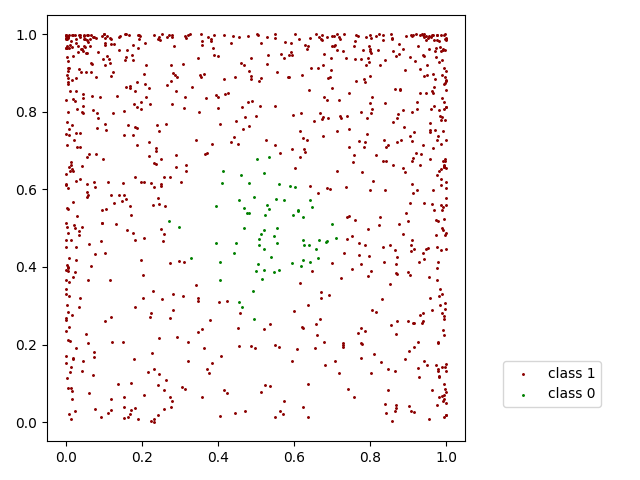
\includegraphics[scale=0.8]{./images/training_data}
  \caption{Training dataset consisting of 1000 samples.}
\end{figure}

Now, for training consider a randomly sampled training set of size $N=1000$, and for $n=m=6$, consider equidistant partitions of the intervals $[0, 1]$. We evaluate the performance of the trained classifier using the metrics \textit{accuracy (acc)}, \textit{true positive rate (tpr)} and \textit{false negative rate (fnr)}.  Using a randomly sampled evaluation dataset consisting of $1500$ samples we get 
\begin{align*}
	acc = 0.956, ~ tpr = 0.9835, ~ fpr = 0.0165.
\end{align*}






        \newpage

    \bibliographystyle{plain}
    \bibliography{myBib}

\end{document}
